%%%%%%%%%%%%%%%%%%%%%%%%%%%%%%%%%%%%%%%%%%%%%%%%%%%%%%%%%%%%%%%%%%%%%%%%%%%%%%%%
%
% Purpose:  Verification part of V&V for the time model
%
% 
%
%%%%%%%%%%%%%%%%%%%%%%%%%%%%%%%%%%%%%%%%%%%%%%%%%%%%%%%%%%%%%%%%%%%%%%%%%%%%%%%%

% \section{Verification}

\subsection{Top-level requirement}

%%% code imported from old template structure
\inspection{Top-level inspection}\label{inspect:TLI}
 This document structure, the code, and associated files have been inspected, 
 and together satisfy requirement \ref{reqt:toplevel}.
 
\subsection{Verification of Dynamic Time}
\test{SIM\_1\_dyn\_only}\label{test:1dynonly}
\begin{description}
\item[Purpose:]\ \newline
To verify that the Dynamic Time functions as a stand-alone implementation of 
time that can be used for integration purposes.

\item[Requirement:]\ \newline
Satisfactory conclusion of this test satisfies requirement 
\ref{reqt:timeinitializationbypass}.

Satisfactory conclusion of this test, along with test 
\ref{test:sim2scalefactor} satisfies requirement \ref{reqt:physicaltime}

\item[Procedure:]\ \newline
A simulation was created with no additional time registrations, and set to run 
such that Dynamic Time = Simulator Time.  No specific time was set, and no 
initialization of any time-types was required.

\item[Predictions:]\ \newline
Dynamic Time should progress with Simulator Time.

\item[Results:]\ \newline
Dynamic Time progressed with Simulator Time.
\end{description}
 
 
 
 
\test{SIM\_2\_dyn\_plus\_STD/RUN\_scale\_factor\_changes/}
\label{test:sim2scalefactor}
\begin{description}
\item[Purpose:]\ \newline
\begin{enumerate}
	\item To test whether Dynamic Time can also operate at some scaled 
	version of Simulator Time.
	\item To test whether that scale factor can be changed mid-simulation, 
	and have Dynamic Time retain its smooth flow.
\end{enumerate}

\item[Requirement:]\ \newline
Satisfactory conclusion of this test, and that of \ref{test:1dynonly}, 
satisfies requirement \ref{reqt:physicaltime}.

\item[Procedure:]\ \newline
A simulation was set running, in which Dynamic Time started synchronized to 
Simulator Time.  At $Simulator Time = 5$, the scale-factor was changed to -1.0 
(corresponding to a time-reversal).  At $Simulator Time = 10$, the scale-factor 
was changed again, to 0.5.  Then, at $Simulator Time = 20$, the scale-factor 
was changed to -2.0.
A Standard Time was also added to this simulation to ensure that the changes to 
Dynamic Time were propagated to Derived Times.

\item[Predictions:]\ \newline
Dynamic Time should increase from 0 seconds to 5 seconds, then fall back to 0
seconds, then increase back to 5 seconds again (but over a longer Simulator Time
interval), then decrease to -5 seconds before the simulation ends at $Simulator 
Time = 25$.  The Standard Time (in this case, TAI) should show the same 
pattern, only over a different range (Standard Times do not typically start at 
0).

\item[Results:]\ \newline
The following three graphs show the progression of Dynamic Time and TAI, as 
expected.

\begin{figure}[htp]
\begin{center}
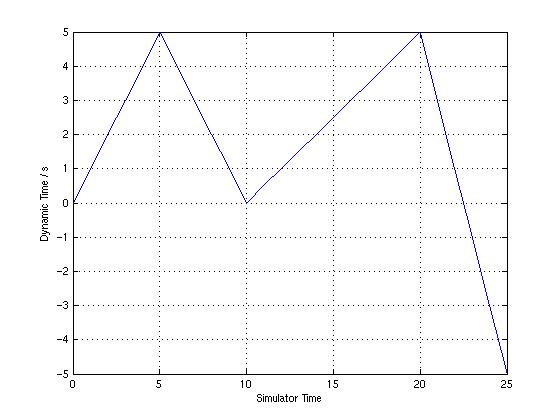
\includegraphics[width=3.2736in,height=2.85in]{figures/sim2_dyn.jpg}
\caption{Variation with Simulator Time of Dynamic Time.}
\end{center}
\end{figure}

\begin{figure}[htp]
\begin{center}
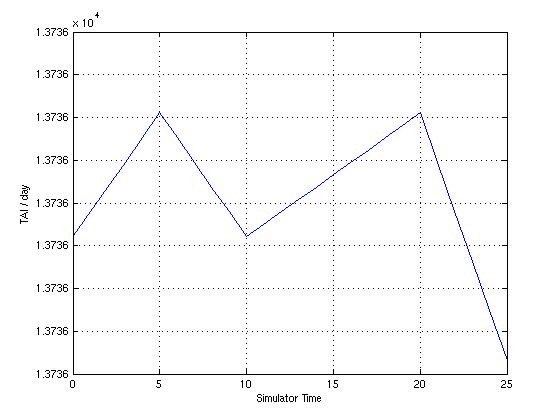
\includegraphics[width=3.2736in,height=2.85in]{figures/sim2_tai.jpg}
\caption{Variation with Simulator Time of TAI.}
\end{center}
\end{figure}

\begin{figure}[htp]
\begin{center}
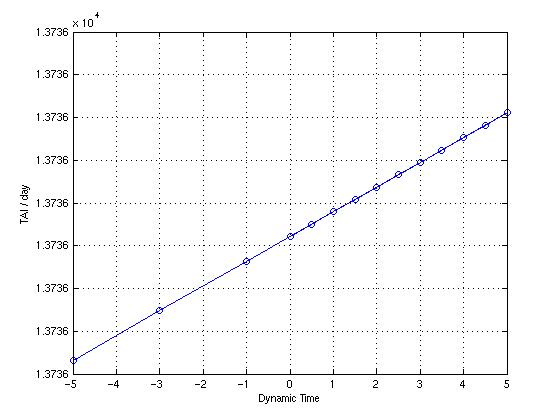
\includegraphics[width=3.2736in,height=2.85in]{figures/sim2_tai_dyn.jpg}
\caption{Variation with Dynamic Time of TAI.}
\end{center}
\end{figure}

\end{description}


\clearpage

\subsection{Verification of Presence of Derived Times and of the Initialization and Propagation Thereof}
\test{SIM\_5\_all\_inclusive/RUN\_UTC\_initialized}  \label{test:clockpresence}
\begin{description}
\item[Purpose:]\ \newline
To ensure that the clocks specified in requirement \ref{reqt:datatimerepresentation} are present and functioning.

\item[Requirement:]\ \newline
Satisfactory conclusion of this test satisfies requirement \ref{reqt:datatimerepresentation}.

Satisfactory conclusion of this test, together with \ref{test:UDEinitbyval} satisfies requirement \ref{reqt:timeinitializationUDE}.


\item[Procedure:]\ \newline
A simulation was developed that contained all clocks included in the release of \JEODid.

\item[Predictions:]\ \newline
All clocks will tick at their appropriate rates, with values consistent with each other.

\item[Results:]\ \newline
All clocks performed as expected.  Figure \ref{fig:sim5} shows the progression of the \textit{calendar\_second} and \textit{clock\_second} values during the simulation.

Some key observations from this plot:
\begin{itemize}
	\item After kicking down to 0 seconds (at the end of the minute), UTC holds for 1 second.  This is an effect of the leap second that was added there.
	\item MET1 is initialized in such a way that the respective values of UTC and MET1 are equivalent up to the addition of the leap second.  Since MET1 is scheduled to update from TAI (and therefore ticks with TAI), it will not have a leap second and will be offset from UTC for all time after the leap second.
	\item MET2 is scheduled to start with a negative value, and to hold during the middle of the simulation.
	\item UT1 advances a little behind UTC; after the leap second, it is a little ahead. 
	\item TDB is not shown; on this scale, it is an overlay of TT.
	\item Data is recorded every second; the last value recorded before the minute ticks over in UTC, UT1, and TT  is the last value in the range [59,60) s, which is not consistent between clocks (as expected).
	
\end{itemize}
  
\begin{figure}[htp]
\begin{center}
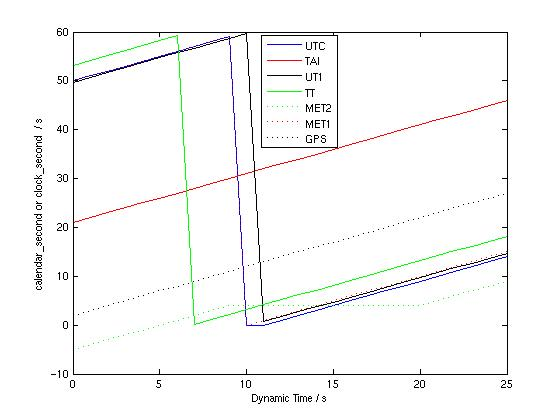
\includegraphics[width=3.2736in,height=2.85in]{figures/sim5_seconds.jpg}
\caption{Variation with Dynamic Time of Derived Times.}\label{fig:sim5}
\end{center}
\end{figure}
  
  

\end{description}














\clearpage




\subsubsection{Verification of TDB to TAI Conversion}

\test{SIM\_5\_all\_inclusive/RUN\_UTC\_initialized\_tdb}  \label{test:UDEinitbytdb}
\begin{description}
\item[Purpose:]\ \newline
To demonstrate that the newly added convert\_b\_to\_a() function correctly implements the
non-trivial conversion algorithm from TDB to TAI.

\item[Requirement:]\ \newline
Satisfactory conclusion of this test satisfies requirement \ref{reqt:timeinitializationrep},
providing the ability for time clocks to be converted to a different type in the reverse direction.

\item[Procedure:]\ \newline
The following entries in the input file were changed:
\begin{verbatim}
	LOG_CYCLE = 1.0
	execfile( "Log_data/log_rec_tdb.py" )

	jeod_time.utc.calendar_year = 2017
	jeod_time.utc.calendar_month = 10
	jeod_time.utc.calendar_day = 28
	jeod_time.utc.calendar_hour = 01.0
	jeod_time.utc.calendar_minute = 23.0
	jeod_time.utc.calendar_second = 45.0
\end{verbatim}
to change the initialization time to match the initialization time of a results comparison python script.
\begin{verbatim}
	jeod_time.tdb.initialize_from_name = "UTC"
\end{verbatim}
to
\begin{verbatim}
	jeod_time.tdb.initialize_from_name = "TAI"
\end{verbatim}
to change from a UTC-initialized simulation to a TAI-initialized simulation.
\begin{verbatim}
	trick.sim_services.exec_set_terminate_time(3600*2)
\end{verbatim}
to allow the simulation to run for two hours.

The following changes were made in the \textit{Log\_data} directory.

Create a new \textit{log\_rec.py} file named \textit{log\_rec\_tdb.py}. In this new file, remove all dr\_group.add\_variable("") lines of code, except for
\begin{verbatim}
	dr_group.add_variable( "jeod_time.tai.calendar_second")
	dr_group.add_variable( "jeod_time.tdb.calender_second")
\end{verbatim}
and change these lines to
\begin{verbatim}
	dr_group.add_variable( "jeod_time.tai.seconds")
	dr_group.add-variable( "jeod_time.tdb.seconds")
\end{verbatim}
This allows only the TAI and TDB variables to be recorded in seconds when the simulation runs.

\item[Predictions:]\ \newline
All clocks will tick at their appropriate rates, with values consistent with each other. Results produced by the simulation and the comparison script should be equal.

\item[Results:]\ \newline
All data consistent with expectations.

\end{description}


\subsection{Verification of Initialization by Derived Times}


\subsubsection{Verification of Initialization by Standard Time}


\test{SIM\_5\_all\_inclusive}  \label{test:STDinitbytype}
\begin{description}
\item[Purpose:]\ \newline
To demonstrate that changes to the identification of which type is the \textit{initializer}, coupled with associated changes to the initialization and update trees, and declaration of appropriate initial values, will result in the simulation being initialized in whichever time-type is desired. 

\item[Requirement:]\ \newline
Satisfactory conclusion of this test, and that of \ref{test:UDEinitbyval}, satisfies requirement \ref{reqt:timeinitializationrep}.

\item[Procedure:]\ \newline
The following entries in the input file were changed:
\begin{verbatim}
	time.manager_init.initializer = "UTC";
	time.utc.calendar_year = 1998;
  time.utc.calendar_month = 12; 
  time.utc.calendar_day = 31; 
  time.utc.calendar_hour = 23; 
  time.utc.calendar_minute = 59; 
  time.utc.calendar_second = 50.0;
\end{verbatim}
by replacing reference to UTC with reference to the desired class.

The initialization and update tree definitions were changed, e.g. from
\begin{verbatim}
  time.tai.initialize_from_name = "UTC";
\end{verbatim}
to 
\begin{verbatim}
  time.utc.initialize_from_name = "TAI";
\end{verbatim}
to change from a UTC-initialized simulation to a TAI-initialized simulation.
  
\item[Predictions:]\ \newline
All clocks should still initialize, but with different values because the initialization time has changed (it is numerically the same, but now on a different clock).
All clocks should progress as before.

\item[Results:]\ \newline
All data was consistent with expectations.

\end{description}




\test{SIM\_2\_dyn\_plus\_STD/initialize\_by\_value}\label{test:STDinitbyval}
\begin{description}
\item[Purpose:]\ \newline
To test the initialization routines, to ensure that a Standard Time can be initialized by a value expressed as a Truncated Julian Time value, a Modified Julian Time value, a Julian Day value, seconds since J2000, or days since J2000.

\item[Requirement:]\ \newline
Satisfactory conclusion of this test, together with test \ref{test:STDinitbycal}, and test \ref{test:UDEinitbyval} satisfy requirements \ref{reqt:timeinitializationbyformat} and \ref{reqt:formattimerepresentation}.

\item[Procedure:]\ \newline
The input file for the run identified as \textit{RUN\_initialize\_by\_value} contains several lines of options.  Each option was tested, one at a time, and the resulting data considered. 

For each option, the simulation was initialized to a value of 10,000 (units correspond to the option).  For each option, the output was plotted as a Truncated Julian Time representation.

\item[Predictions:]\ \newline
\begin{itemize}
	\item {Truncated Julian Time}
	
	The output should have a value of $10,000$ days.
	\item {Modified Julian Time}
	
	Modified Julian Time differs from truncated Julian Time by 40,000 days.  If Modified Julian Time = $10,000$ days, then Truncated Julian Time = $-30,000$ days.
	\item {Julian Time}
	
	Julian Time differs from Truncated Julian Time by 2,440,000.5 days.  If Julian Time = $10,000$ days, then Truncated Julian Time = $-2.4300005 \times 10^6 $ days.
	\item {seconds\_since\_epoch}
	
	The TAI epoch is set to J2000, corresponding to a Truncated Julian Time of $11544.4996275$ days in TAI.  $10,000$ seconds (or $0.11574$ days) after this point gives Truncated Julian Time = $11544.61536824074$ days.
	\item {days\_since\_epoch}
	
	10,000 days after the TAI epoch has a Truncated Julian Time of $21544.4996275$ days.
\end{itemize}

\item[Results:]\ \newline
  All values agreed with their predicted values.
\end{description}





\test{SIM\_2\_dyn\_plus\_STD/RUN\_initialize\_by\_calendar}  \label{test:STDinitbycal}
\begin{description}
\item[Purpose:]\ \newline
To test whether a Standard Time can be correctly initialized by a calendar representation.

\item[Requirement:]\ \newline
Satisfactory conclusion of this test, together with test \ref{test:STDinitbyval}, and test \ref{test:UDEinitbyval} satisfy requirement \ref{reqt:timeinitializationbyformat}.


\item[Procedure:]\ \newline
A simulation was created comprising Dynamic Time and TAI.  The initialization was set to a calendar value of 2005/12/31::23:59:50.0 TAI. 

\item[Predictions:]\ \newline
The calendar value should correspond to a Truncated Julian Time of 13735.9998842593

\item[Results:]\ \newline
The predicted value is correct.

\end{description}



\subsubsection{Verification of Initialization by User-defined-epoch Times}


\test{SIM\_5\_all\_inclusive/RUN\_UDE\_initialized}  \label{test:UDEinitbyval}
\begin{description}
\item[Purpose:]\ \newline
To test whether the \timeDesc\ can be initialized from a UDE time-type, using either an initial value, or a clock.

\item[Requirement:]\ \newline
Satisfactory conclusion of this test, together with test \ref{test:STDinitbycal}, and test \ref{test:STDinitbyval} satisfies requirement \ref{reqt:timeinitializationbyformat}.

Satisfactory conclusion of this test, together with test \ref{test:STDinitbytype}, satisfies requirement \ref{reqt:timeinitializationrep}.

Satisfactory conclusion of this test, together with test \ref{test:clockpresence}, satisfies requirement \ref{reqt:timeinitializationUDE}.




\item[Procedure:]\ \newline
In the all-inclusive simulation with an initialization by a UDE, there are two options for initializing the UDE (and hence the simulation).  One is by using the initial value of the UDE in \textit{seconds\_since\_epoch}, and the other by specifying a clock format (still representing time since epoch).  The same simulation was run with both options.

\item[Predictions:]\ \newline
The two runs should produce identical results, and the other time representations should generate data consistent with a simulation starting at 1998/12/31::23:59:50.0.

\item[Results:]\ \newline
The data are as expected.
\end{description}


\subsection{Verification of Data Over-rides}
\test{SIM\_4\_common\_usage/RUN\_JEOD1x\_compatible}  \label{test:overrides}
\begin{description}
\item[Purpose:]\ \newline
To ensure that the methods can be used for simulations set in the future for which data values are not included in the \JEODid\ release, and to demonstrate a method by which the \JEODid\ data output can be compared directly against that from previous releases.

\item[Requirement:]\ \newline
Satisfactory conclusion of this test satisfies requirement \ref{reqt:backwardcompatibility}.

\item[Procedure:]\ \newline
The flags \textit{true\_utc} and \textit{true\_ut1} were forced to false, effectively eliminating the capability of updating the offset values from the most recent data.  Instead, an offset between, say TAI and UTC, will be calculated initially, and that value will remain as a constant for the duration of the simulation.

\item[Predictions:]\ \newline
Running through the known instant of a leap second will produce no effect on UTC with the flags turned off.  The two UT1 values (with flag set to true and false) will be identical at the start of the simulation, and gradually diverge throughout the simulation.

\item[Results:]\ \newline
The data are as expected.
In the following figure legends, ``***-1'' refers to the JEOD1.x compatible
data, and ``***-2'' refers to the data obtained with the default settings in \JEODid.
Figure \ref{fig:sim4all} shows the relation between TAI, UTC, and UT1 at a time near the end of the simulation.  

Figure \ref{fig:sim4leap} represents a small part of figure \ref{fig:sim4all}, zoomed in. It shows the separation of the two UTC values at the point at which a leap second is encountered (Note that the leap second is added to the \JEODid\ version of UTC, and the JEOD1 version of UTC keeps ticking right through it).  

Figure \ref{fig:sim4ut1} represents a further zoom in, and shows the difference between the two UT1 times.

Finally, figure \ref{fig:sim4dut1} shows the difference between the two UT1 values clearly growing over time.  A similar plot differencing the two UTC values is not presented, it showed a flat line 0 preceding the leap second; thereafter, the difference was 1 second, except as the minutes ticked over, when it would jump to 59 seconds (because one time would tick over and go to zero while the other was still near 60).

\begin{figure}[htp]
\begin{center}
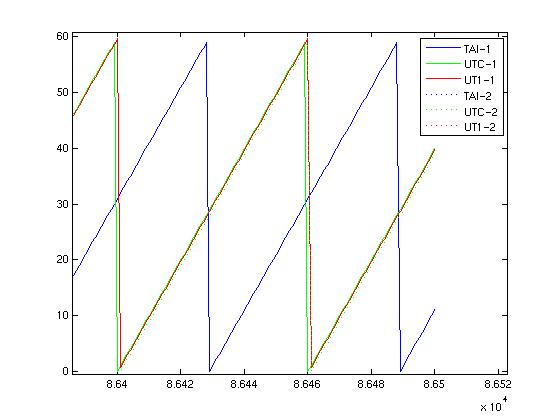
\includegraphics[width=3.2736in,height=2.85in]{figures/sim4_all.jpg}
\caption{Showing the relation between TAI, UTC, and UT1.}\label{fig:sim4all}
\end{center}
\end{figure}
\begin{figure}[htp]
\begin{center}
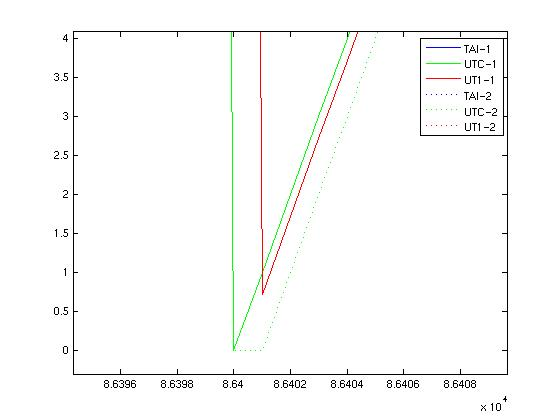
\includegraphics[width=3.2736in,height=2.85in]{figures/sim4_leap.jpg}
\caption{Values of UTC showing the addition of a leap second in the \JEODid-compatible version, but not in previous versions.}\label{fig:sim4leap}
\end{center}

\end{figure}
\begin{figure}[htp]
\begin{center}
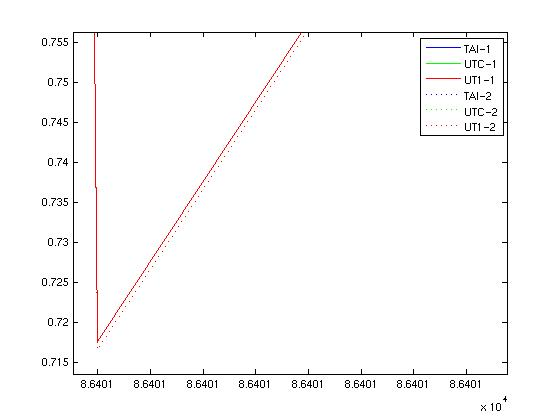
\includegraphics[width=3.2736in,height=2.85in]{figures/sim4_ut1_end.jpg}
\caption{Values of UT1 showing the difference between performing regular updates and using a fixed data-file override value.  This difference is after approximately 1 day of Dynamic Time.}\label{fig:sim4ut1}
\end{center}

\end{figure}
\begin{figure}[htp]
\begin{center}
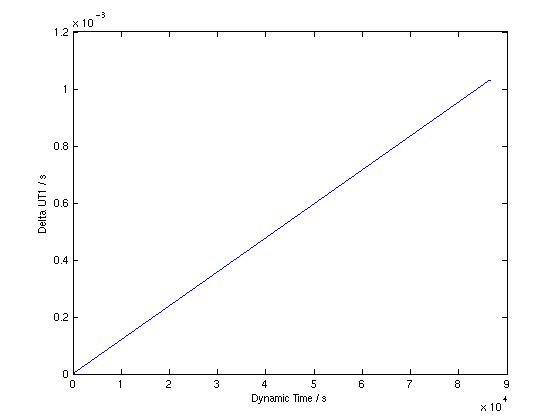
\includegraphics[width=3.2736in,height=2.85in]{figures/sim4_deltaut1.jpg}
\caption{The difference,over a period of 1 day, between the values of UT1 using a regular update, versus using a fixed data-file override value.}\label{fig:sim4dut1}
\end{center}
\end{figure}
\end{description}

\clearpage

\subsection{Verification of Extension Capabilities}
\test{SIM\_6\_extension}  \label{test:sim6}
\begin{description}
\item[Purpose:]\ \newline
To ensure that new clocks and converters can be added without altering the
existing code-base.

\item[Requirement:]\ \newline
Satisfactory conclusion of this test satisfies requirement
\ref{reqt:extensibility}.

\item[Procedure:]\ \newline
A new clock and accompanying converter were added to the simulation, as
described in the \textref{User Guide}{sec:User_Extension}.

\item[Predictions:]\ \newline
The time would evolve as Dynamic Time progresses.

\item[Results:]\ \newline
The data are as expected.
\end{description}
